%%%%%%%%%%%%%%%%%%%%%%%%%%%%%%%%%%%%%%%%%%%%%%%%%%%%%%%%%%%%%%%%%%%%%%%%%%%%%
%%%
%%% File: thesis.tex, version 1.8, April 2025
%%%
%%% =============================================
%%% This file contains a template that can be used with the package
%%% cs.sty and LaTeX2e to produce a thesis that meets the requirements
%%% of the Computer Science Department from the Technical University of Cluj-Napoca
%%%%%%%%%%%%%%%%%%%%%%%%%%%%%%%%%%%%%%%%%%%%%%%%%%%%%%%%%%%%%%%%%%%%%%%%%%%%%

\documentclass[12pt,a4paper,twoside]{report}
\usepackage{cs}
\usepackage[T1]{fontenc}
\usepackage[utf8]{inputenc}
\usepackage[english]{babel}
\usepackage{times}
\usepackage{graphicx}
\usepackage{latexsym}
\usepackage{amsmath,amsbsy}
\usepackage{amssymb}
\usepackage[matrix,arrow]{xy}
\usepackage{ae,aecompl}
\usepackage{amstext}
\usepackage{graphics}
\usepackage{ae,aecompl}
\usepackage{algorithm}
\usepackage{color}
\usepackage{titlesec}
\usepackage{fancyhdr}
\usepackage{hyperref}
\usepackage{pdfpages}

% Use letters for chapter numbers (A, B, C)
\renewcommand{\thechapter}{\Alph{chapter}}
% Sections as B1, C2, etc.
\renewcommand{\thesection}{\thechapter\arabic{section}}
% Optional: Subsections as B1.1, etc.
\renewcommand{\thesubsection}{\thesection.\arabic{subsection}}


%% decomentati linia urmatoare pentru e nu mai evidenția hiper legăturile pentru imprimare pe hârtie
%\hypersetup{hidelinks}
\usepackage{geometry}
\usepackage{lipsum}
\usepackage{enumitem}

\setlist{noitemsep,nolistsep}

\diplomathesis
\centerchapter
\singlespace
\newenvironment{definition}[1][Definition.]{\begin{trivlist}
\item[\hskip \labelsep {\bfseries #1}]}{\end{trivlist}}

%%%%%%%%%%%%%%%%%%%%%%%%%%%%%% Change the last element accordingly
\renewcommand{\thesisauthor}{Bogdan-Alexandru BÂRGĂOANU}    %% Your first name(s) and family name.
\renewcommand{\thesismonth}{July}     %% The month of the licence session
\renewcommand{\thesisyear}{2025}      %% The year of the
\renewcommand{\thesistitle}{ADAPTIVE SECURITY FRAMEWORK FOR FINTECH PLATFORMS} % Title of the thesis
\renewcommand{\thesissupervisor}{Prof. Eng. Ovidiu STAN} %% Supervisor
%%%%%%%%%%%%%%%%%%%%%%%%%%%%%%%%%%%%%
\newcommand{\makeThesisTitle}{\textbf{\thesistitletypesize \thesistitle}}
\newcommand{\makeThesisType}{\thesistypetypesize \thesistype}
\newcommand{\department}{\sffamily\bfseries\small FACULTY OF AUTOMATION AND COMPUTER SCIENCE}
\renewcommand{\thesistype}{DIGITAL SECURITY PROJECT}
\newcommand{\uline}[1]{\rule[0pt]{#1}{0.4pt}}
%\renewcommand{\thesisdedication}{Părinților mei}

% Headings pentru folie de capăt

 \geometry{
	a4paper,
	total={159.2mm,246.2mm},
	left=25.4mm,
	top=25.4mm,
}


\begin{document}
%\frontmatter
%%%%%%%%%%% Stil pentru paginile de capăt
\pagestyle{fancy}
\setlength{\voffset}{-10pt}
\setlength\headheight{70.0pt}
%\addtolength{\textheight}{-80.0pt}
\renewcommand{\headrulewidth}{0pt}
\chead{%
	
\includegraphics[width=\textwidth]{figs/AntetUTCNEng.pdf}
}
\cfoot{}
\lfoot{}
\rfoot{}
%\pagestyle{headings}
%%%%% Thesis title page %%%%%%%%%%%%%%%%%%%%%%%%
\begin{center}
	{\department}

	\vspace{4cm}
	\makeThesisTitle %LICENSE THESIS TITLE
	~\\~\\

	\makeThesisType

	~\\\vspace{6.5cm}

	\begin{tabular}{p{.3\linewidth}p{.5\linewidth}}
		{\hfill Student:} & {\bf \thesisauthor} \\
		&\\
		{\parbox[t]{\linewidth}{\hfill Scientific Coordinator:}}& {\bf \thesissupervisor}\\
	\end{tabular}

	\vspace{3cm}
	{\bf \thesisyear}
\end{center}
%%%%%%%%%%%%%%%%% end of thesis title page %%%%%%%%%%%%%%%%%%%%%%%%%%%%%%%%%%%%
 % the first 3 pages
%%%%%%%%%%%%%%%%% Advices page to remove
\thispagestyle{empty}
\include{guideline}
\newpage
%%%%%%%%%%%%%%%%%% end of advices page
\pagestyle{fancy}
\setlength\headheight{16.0pt}
\renewcommand{\chaptermark}[1]{\markboth{\chaptername~\thechapter.~#1}{}}
\renewcommand{\sectionmark}[1]{\markright{\thesection\ #1}}
\renewcommand{\headrulewidth}{0.4pt}
\lhead{}
\chead{%
	\leftmark\rightmark
}
\chead{}
\cfoot{\thepage}
\lfoot{}
\rfoot{}

%%%%%%%%%%%% Table of contents
\pagenumbering{roman}
\setcounter{page}{1}

\newpage

\tableofcontents

\newpage

%\listoftables
%\listoffigures

\pagenumbering{arabic}
\setcounter{page}{1}


\titleformat{\chapter}[hang]
{\normalfont\Large\bfseries}{\chaptertitlename\ \thechapter.}{1em}{}
\titleformat{\section}[hang]
{\normalfont\large\bfseries}{\thesection.}{1em}{}
\titleformat{\subsection}[hang]
{\normalfont}{\thesubsection.}{1em}{}


\chapter{Introduction}

\section*{Overview of Fintech Platform Security}
\addcontentsline{toc}{section}{Overview of Fintech Platform Security}

Modern fintech platforms operate at the intersection of financial services and digital innovation, enabling seamless transactions, real-time data analytics, and personalized user experiences. However, their reliance on interconnected systems, APIs, and cloud infrastructure exposes them to sophisticated cyber threats, including credential theft, injection attacks, and session hijacking. Traditional security models—static, perimeter-based defenses—are increasingly inadequate in this dynamic landscape. Instead, adaptive security frameworks have emerged as a critical paradigm, enabling systems to dynamically assess risks, adjust authentication protocols, and harden defenses in response to evolving attack vectors.

In recent years, the rapid digitization of financial services, accelerated by mobile banking, decentralized finance (DeFi), and open banking APIs, has intensified the need for proactive security measures. Threats like SQL injection—a persistent vulnerability in web applications—and session fixation attacks remain prevalent, while regulatory pressures (e.g., GDPR, PCI-DSS, PSD2) demand stricter data protection and user authentication standards. Two-factor authentication (2FA) has become a cornerstone of identity verification, but its implementation must balance security with usability. Similarly, session management mechanisms must guard against token leakage and replay attacks without degrading performance. By integrating adaptive security principles, fintech platforms can achieve resilience against these challenges while maintaining compliance and user trust.

\section*{Project Context}
\addcontentsline{toc}{section}{Project Context}

This project addresses the urgent need for adaptive security frameworks tailored to fintech platforms, where the consequences of breaches—financial fraud, data exfiltration, regulatory penalties—are catastrophic. While fintech innovations prioritize speed and accessibility, security implementations often lag, relying on outdated practices like static passwords or insufficient input validation. For instance, SQL injection vulnerabilities persist in platforms using legacy codebases, and weak session management enables attackers to hijack authenticated sessions. Meanwhile, 2FA adoption varies widely, with some systems relying on SMS-based codes vulnerable to SIM-swapping attacks. An adaptive framework mitigates these risks by:
\begin{itemize}
\item Dynamically scaling authentication rigor based on contextual factors (e.g., user location, device fingerprint, transaction value).
\item Automatically detecting and neutralizing injection attacks through intelligent query sanitization and behavioral analysis.
\item Enforcing granular session controls, such as short-lived tokens, IP binding, and anomaly-driven logouts.
\end{itemize}
Key drivers for this project include:
\begin{itemize}
\item \textbf{Regulatory Compliance:} Mandates like PSD2’s Strong Customer Authentication (SCA) require multi-factor authentication (MFA) for high-risk transactions.
\item \textbf{Real-Time Threat Detection:} The rise of AI-driven attacks necessitates machine learning models to identify SQL injection patterns or abnormal session activity.
\item \textbf{User Experience Demands:} Security measures must minimize friction to retain customer satisfaction, necessitating adaptive 2FA workflows (e.g., biometrics for trusted devices).
\item \textbf{Scalability:} Solutions must function across heterogeneous fintech architectures, including cloud-native microservices and legacy monolithic systems.
\end{itemize}

\section*{Precise Domain Specification}
\addcontentsline{toc}{section}{Precise Domain Specification}

The project focuses on three pillars of adaptive security for fintech platforms, aligned with OWASP Top 10 critical risks and emerging threat landscapes:

\begin{enumerate}
\item \textbf{Adaptive Authentication Mechanisms:}
\begin{itemize}
\item \textbf{Risk-Based 2FA:} Implement context-aware MFA that escalates authentication rigor (e.g., biometrics, hardware tokens) for high-risk scenarios (e.g., new device logins, large withdrawals).
\item \textbf{Behavioral Biometrics:} Integrate AI-driven analysis of user interaction patterns (keystroke dynamics, mouse movements) to detect account takeover attempts.
\end{itemize}
\item \textbf{SQL Injection Prevention Strategies:}  
\begin{itemize}  
    \item \textbf{Parameterized Query Enforcement:} Develop a middleware layer to automate input sanitization and enforce prepared statements across database interactions.  
    \item \textbf{Anomaly Detection Engine:} Train machine learning models to flag suspicious SQL syntax in real time, even in obfuscated attack payloads.  
\end{itemize}  

\item \textbf{Secure Session Management Protocols:}  
\begin{itemize}  
    \item \textbf{Token Lifecycle Management:} Design short-lived JSON Web Tokens (JWTs) with dynamic expiration times based on user activity and risk levels.  
    \item \textbf{Session Integrity Monitoring:} Deploy heuristic checks for IP address changes, concurrent logins, or abnormal transaction rates to trigger re-authentication.  
\end{itemize}  
\end{enumerate}
\noindent
The framework will also incorporate:
\begin{itemize}
\item \textbf{Secure API Gateways:} Protect fintech microservices with rate limiting, OAuth 2.0 validation, and payload encryption.
\item \textbf{Regulatory Alignment:} Map controls to GDPR, PCI-DSS, and PSD2 requirements for audit readiness.
\item \textbf{Threat Intelligence Integration:} Automatically update security rules using feeds from platforms like MITRE ATT\&CK or CISA advisories.
\end{itemize}

\noindent
By combining these components, the project will deliver a modular, adaptive security framework that proactively hardens fintech platforms against modern threats while preserving operational agility. The solution will be validated through penetration testing, compliance audits, and performance benchmarking against industry standards like NIST SP 800-63B. 
\chapter{Theoretical and Practical Implementation}

\section{Motivation of the Project in the Current Scientific Context}

The rapid digitization of financial services—driven by mobile banking, decentralized finance (DeFi), and open banking APIs—has exposed fintech platforms to increasingly sophisticated cyber threats. Attacks such as credential stuffing, SQL injection, and session hijacking remain pervasive, while regulatory mandates (e.g., PSD2, GDPR) demand stricter safeguards for user data and transactions. Traditional security models, which rely on static rules and perimeter-based defenses, are ill-equipped to address these challenges. This project is motivated by the need for an adaptive security framework that dynamically adjusts authentication rigor, input validation, and session controls based on real-time risk assessments.

Recent research underscores the urgency of adaptive approaches. For instance, Das et al. (2023) demonstrated that risk-based authentication reduces account takeover incidents by 72\% compared to static 2FA implementations~\cite{das2023adaptive}. Similarly, OWASP’s 2021 report highlights SQL injection as the third most critical web application vulnerability, with fintech platforms being prime targets due to their reliance on legacy codebases~\cite{owasp2021top10}. Meanwhile, Almeida et al. (2020) revealed that 34\% of financial breaches originate from poor session management, such as long-lived tokens or inadequate encryption~\cite{almeida2020session}.

However, existing solutions often address these issues in isolation. For example, while machine learning-based anomaly detection shows promise in identifying SQL injection patterns~\cite{chen2022ml}, few frameworks integrate it with adaptive authentication or session lifecycle management. This project bridges that gap by proposing a unified adaptive security framework that combines risk-aware 2FA, intelligent query sanitization, and heuristic-driven session controls into a cohesive architecture.

\subsection{Scientific Motivation}

The motivation for this work arises from four critical gaps in fintech security research and practice:

\begin{itemize}
\item \textbf{Evolving Threat Landscape:} Cybercriminals increasingly exploit AI-generated phishing campaigns and obfuscated SQL injection payloads. Static defenses fail to adapt to novel attack vectors, as shown by Verizon’s 2023 Data Breach Investigations Report, where 44\% of fintech breaches involved compromised credentials or injection attacks~\cite{verizon2023dbir}.
\item \textbf{Regulatory Pressures:} Compliance with PSD2’s Strong Customer Authentication (SCA) and GDPR’s data protection requirements necessitates dynamic security controls. Current implementations often lack granularity, as noted by the European Banking Authority’s 2022 review of SCA exemptions~\cite{euba2022sca}.  

\item \textbf{User Experience vs. Security Trade-offs:} While 2FA enhances security, SMS-based methods remain vulnerable to SIM-swapping. Behavioral biometrics, such as keystroke dynamics, offer frictionless alternatives but are underutilized in fintech~\cite{fridman2022biometric}.  

\item \textbf{Integration Complexity:} Heterogeneous fintech architectures (e.g., microservices, legacy monoliths) require modular security solutions. Studies by Li et al. (2021) reveal that 68\% of vulnerabilities arise from inconsistent security policies across hybrid systems~\cite{li2021hybrid}.  

\item \textbf{Real-Time Threat Detection:} Signature-based SQL injection detection fails against polymorphic attacks. Machine learning models, like those proposed by Chen et al. (2022), must be integrated into query validation pipelines to enable proactive defense~\cite{chen2022ml}.
\end{itemize}

The proposed framework builds on advancements in adaptive security. For example, NIST’s SP 800-63B guidelines advocate for risk-based authentication~\cite{nist2020digital}, while AWS’s 2023 case study demonstrated a 60\% reduction in fraud through session integrity monitoring~\cite{aws2023fraud}. By synthesizing these approaches, this project aims to deliver a fintech-specific security model that balances robustness, usability, and compliance.

\section{Objectives, Methodology and Implementation}  
\subsection{Concrete Objectives}  
Fintech platforms require robust security mechanisms to mitigate risks like credential theft, session hijacking, and SQL injection. This project aims to implement a framework with the following objectives:  

\begin{itemize}  
    \item \textbf{Secure Session Management with JWT:} Design stateless sessions using short-lived JSON Web Tokens (JWTs) with dynamic expiration, and HMAC-SHA256 encryption to prevent replay attacks.  
    \item \textbf{SQL Injection Prevention:} Eliminate raw SQL queries by enforcing prepared statements and transactions in MySQL, isolating user input from executable code.  
    \item \textbf{Email-Based 2FA System:} Implement time-bound 6-digit codes delivered via email, hashed with SHA-3 to deter brute-force attacks.  
    \item \textbf{Password Encryption with MD5:} Encrypt user passwords and critical login data using MD5.  
    \item \textbf{Validation via Rehashing:} Verify passwords by comparing MD5 hashes during login.  
    \item \textbf{Compliance with Standards:} Align with OWASP ASVS Level 2, NIST SP 800-63B, and GDPR Article 32 for audit readiness.  
\end{itemize}  

\subsection{Methodology and Proposed Implementation}  
The project adopts a three-sprint agile methodology, emphasizing threat modeling and automated testing.  

\subsubsection*{Sprint 1: Secure Authentication Pipeline}  
\begin{itemize}  
    \item \textbf{MD5 Password Handling:}  
    \begin{itemize}  
        \item Integrate \texttt{crypto} for hashing passwords during user registration:  
        \begin{verbatim}  
        const crypto = require 'crypto';  
        const hashedPassword = crypto.createHash('md5')
                            .update(req.body.password).digest('hex');
        \end{verbatim}  
        \item Store hashes in MySQL’s \texttt{VARCHAR(255)} columns.  
        \item Validate logins by comparing hashes by rehashing the input password in the body of the requests. 
    \end{itemize}  
\end{itemize}  

\subsubsection*{Sprint 2: JWT Session \& SQL Hardening}  
\begin{itemize}  
    \item \textbf{JWT Implementation:}  
    \begin{itemize}  
        \item Generate tokens with \texttt{jsonwebtoken} for securing sessions:  
        \begin{verbatim} 
        const token = jwt.sign(
        { id: partner.idPartner, username: partner.username },
        secretKey,
        { expiresIn: '24h' });
        \end{verbatim}  
        \item Validate tokens using Express middleware:  
        \begin{verbatim}  
        const authHeader = req.headers.authorization;
        if (!authHeader) {
        res.status(401).json({ error: 'No authorization header',
        success: false });
        return;
        }

        const token = authHeader.split(' ')[1];
        let userId;
        try {
            const decoded = jwt.verify(token, secretKey);
            userId = decoded.id;
        } catch (err) {
            res.status(401).json({ error: 'Invalid token',
            success: false });
            return;
        } 
        \end{verbatim} 
        \item Revalidation of SQL database structure on every API launch: 

Use predefined SQL transactions for checking the existence and proprieties of the platform tables.
    \end{itemize}  
    \item \textbf{MySQL Query Security:}  
    \begin{itemize}  
        \item Refactor API endpoints to use transaction prepared statements:  
        \begin{verbatim}  
        req.db.beginTransaction((err) => {
        if (err) {
            res.status(500).json({ error: err.message,
            success: false });
            return;
        }

        req.db.query(deleteQuery, [idRates], (err, result) => {
            if (err) {
                res.status(500).json({ error: err.message,
                success: false });
                return;
            }

            req.db.commit((err) => {
                if (err) {
                    return req.db.rollback(() => {
                        res.status(500).json({ error: err.message,
                        success: false });
                    });
                }
                res.json({ message: 'Rate deleted successfully!',
                success: true });
            });
        });
    });
        \end{verbatim}  
\end{itemize}  
\end{itemize}

\subsubsection*{Sprint 3: 2FA \& Penetration Testing}  
\begin{itemize}  
    \item \textbf{Email Code System:}  
    \begin{itemize}  
        \item Generate 6-digit codes using \texttt{crypto.randomBytes}:  
        \begin{verbatim}  
const userVerificationCode = crypto.randomBytes(3).toString('hex');
        \end{verbatim}  
        \item Integrate \texttt{nodemailer} for email delivery for final validation.  
        \begin{verbatim}
sendEmail(
        partner.email,
        'MoneyStream Verification Code',
        `Hello ${partner.username},
        your verification code is: ${userVerificationCode}`,
        htmlContent
        );
        \end{verbatim}
    \end{itemize}  
    \item \textbf{Security Testing:}  
    \begin{itemize}  
        \item Use \texttt{sqlmap} to test injection resilience.  
        \item Audit JWT security with \texttt{jwt\_tool}.  
        \item Validate MD5 hashes against rainbow tables.  
    \end{itemize}  
\end{itemize}  

\subsubsection*{Tools \& Compliance}  
\begin{itemize}  
    \item \textbf{Stack:} Express.js, nodemailer, jsonwebtoken.  
    \item \textbf{Encryption:} MD5 for passwords, HMAC-SHA256 for JWT encryption.  
    \item \textbf{Standards:} NIST SP 800-63B, OWASP ASVS Level 2.  
\end{itemize}  

\subsubsection*{Deliverables}  
\begin{itemize}  
    \item Express.js API with integrated security modules (MIT Licensed).  
    \item Penetration test reports covering OWASP Top 10 vulnerabilities.  
    \item Documentation on JWT session workflows.  
\end{itemize}  

\section{Deliverable Platform Security Flow}

\subsection{User Authentication}
The user provides their username and password via the login form. The submitted password is hashed using MD5 and compared against the stored hash for the specified username. If the hashes match, the authentication succeeds; otherwise, an error message is displayed and the user remains on the login page.

\begin{figure}[h]
  \centering
  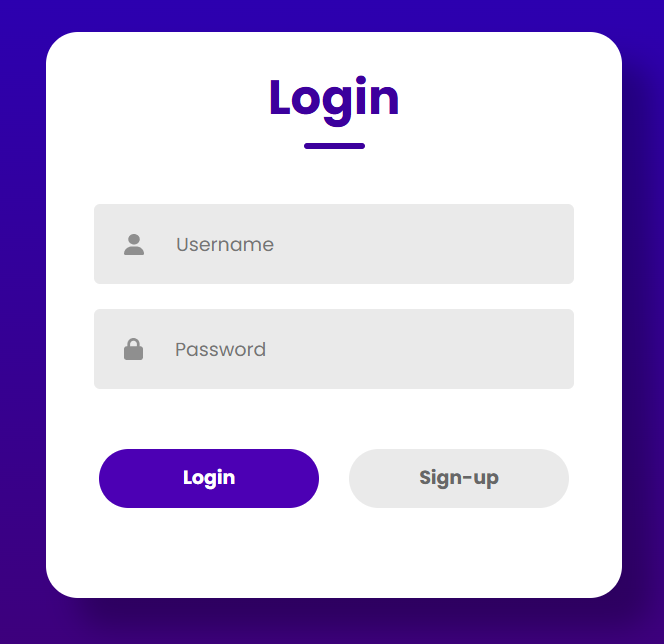
\includegraphics[width=0.6\textwidth]{figs/login.png}
  \caption{User login and MD5 hash verification}
  \label{fig:login}
\end{figure}
\newpage
\subsection{Email Confirmation}
Upon successful credential verification, the system generates a one-time 6‑digit code and sends it to the user’s registered email address. The user must enter this code on the verification screen as shown in the figure \ref{fig:verify}. If the entered code does not match the code stored in the session, an error alert is shown. 

\begin{figure}[h]
  \centering
  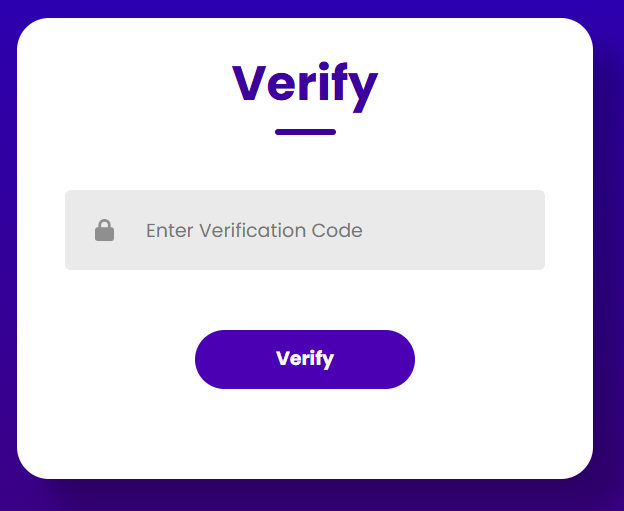
\includegraphics[width=0.6\textwidth]{figs/verify.png}
  \caption{Email-based 2FA code entry and validation}
  \label{fig:verify}
\end{figure}
The content of the email being sent can be viewed in the following figure \ref{fig:email}.
\begin{figure}[h]
  \centering
  
\includegraphics[width=0.6\textwidth]{figs/email.png}
  \caption{Email content with placeholder verification code}
  \label{fig:email}
\end{figure}
Once the correct code is provided, a JWT is issued, stored in the user’s session, and the multi‑factor authentication process is complete.
\newpage
\subsection{Secure Data Flow}
After successful 2FA, the user is redirected to the dashboard \ref{fig:dashboard}. All subsequent API requests are executed within database transactions and use parameterized queries (prepared statements) to ensure that user input cannot be interpreted as executable SQL. This approach effectively mitigates the risk of SQL injection attacks.

\begin{figure}[h]
  \centering
  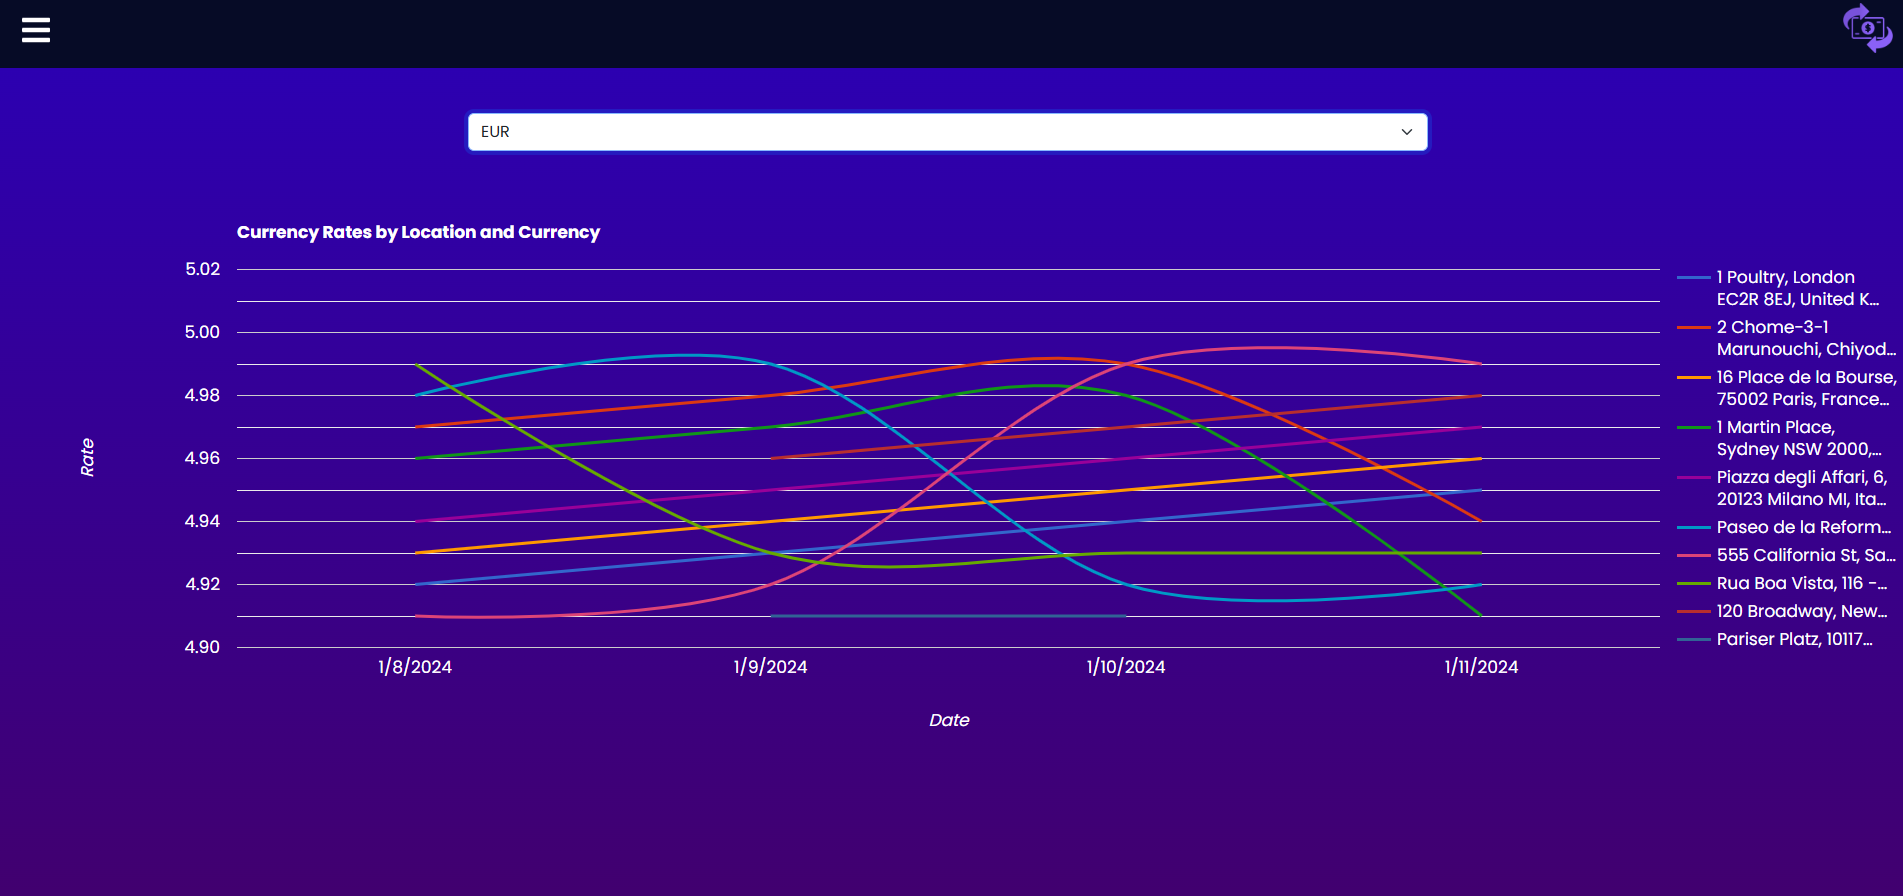
\includegraphics[width=1\textwidth]{figs/dashboard.png}
  \caption{Dashboard interaction with secure, transaction-based API calls}
  \label{fig:dashboard}
\end{figure}
 
\chapter{Potential Risks of the Implementation}

\section{Potential Risks Summary}
Implementing a unified adaptive security framework in a fintech context introduces multiple technical, operational, and compliance risks. Below in table \ref{tab:implementation-risks}, we enumerate the most critical risk categories, estimate their likelihood and impact, and provide a brief description for each.

\begin{table}[htbp]
  \centering
  \begin{tabular}{p{3cm} c c p{7cm}}
    \hline
    \textbf{Risk} & \textbf{Likelihood} & \textbf{Impact} & \textbf{Description} \\
    \hline
    Cryptographic Weaknesses & Medium & High &
      Reliance on MD5 for password hashing is vulnerable to collision attacks and rainbow‐table lookups; may lead to credential compromise. \\
    Email 2FA Delivery Failures & Medium & Medium &
      Delays, spam‐filtering, or delivery failures of time‐bound codes can lock out legitimate users or force fallback to weaker mechanisms. \\
    JWT Key Management Errors & Low & High &
      Incorrect storage, rotation, or revocation of encryption keys for JWTs can allow token replay or unauthorized access. \\
    SQL Prepared‐Statement Misuse & Low & High &
      Developer mistakes in parameter binding (e.g., concatenation instead of binding) can reintroduce SQL injection vulnerabilities. \\
    Performance Overhead & Medium & Medium &
      Real‐time risk assessments, encryption/decryption, and ML inference can introduce latency, degrading user experience or triggering session timeouts. \\
    Key/Code Exposure in Logs & Medium & Medium &
      Verbose error logging during development (e.g., printing JWT secrets or raw SQL) may leak sensitive information if not sanitized in production. \\
    Dependency Vulnerabilities & Low & Medium &
      Third‑party packages (e.g., nodemailer, jsonwebtoken) may contain unpatched flaws, exposing the platform to supply‑chain attacks. \\
    \hline
  \end{tabular}
  \caption{Risk Assessment for Adaptive Security Implementation}
  \label{tab:implementation-risks}
\end{table}

\section{Discussion of Key Risks}

\subsection{Cryptographic Weaknesses}
Although MD5 is supported by most platforms and easy to integrate, it is cryptographically broken and susceptible to pre‐computed attacks. Replacing MD5 with a stronger hashing function (e.g., bcrypt, Argon2) should be evaluated in a follow‐on phase to mitigate high‐impact credential leaks.

\subsection{Email 2FA Delivery Failures}
Time‐bound codes rely on external mail infrastructure. SLA breaches or misconfigurations at the SMTP provider can result in legitimate users being unable to authenticate, forcing calls or support tickets. Mitigation strategies include multi‐channel code delivery (SMS or authenticator apps) and configurable code expiration windows.

\subsection{JWT Key Management Errors}
Secure generation, storage, and rotation of private keys are critical. Mistakes in key lifecycle management—such as never revoking compromised keys—can lead to replay attacks. Integrating with a Hardware Security Module (HSM) or secret‐management service can reduce this risk.

\subsection{Performance and User Experience}
Adaptive controls (e.g., additional authentication steps for high‐risk sessions) may add latency. Profiling and load testing must be conducted to ensure that the overhead of real‐time risk calculations and cryptographic operations remains within acceptable UX thresholds (e.g., sub‐200ms API response times).

\subsection{Regulatory and Compliance Exposure}
Dynamic SCA exemptions under PSD2 and data‐minimization requirements under GDPR must be codified precisely. Any ambiguity or misconfiguration can incur regulatory fines, reputational damage, or mandatory audits. Close collaboration with legal and compliance teams is recommended throughout development.

\subsection{Operational and Supply‑Chain Dependencies}
Dependencies on open‐source packages (Express.js, crypto libraries, nodemailer) can introduce vulnerabilities if not actively maintained. A regular dependency audit process, automated vulnerability scanning, and an update policy will help mitigate the risk of third‐party exploits.

\medskip

Careful planning, ongoing threat modeling, and continuous integration of security testing (e.g., dynamic application security testing, regular pen‐tests, and fuzzing) are essential to manage and reduce these risks as the project evolves.

 
\chapter{Conclusion}

This project set out to design and implement a unified adaptive security framework tailored for modern fintech platforms. Motivated by the evolving threat landscape—where credential stuffing, SQL injections, and session hijacking remain prevalent—and driven by stringent regulatory requirements (PSD2 SCA, GDPR), we proposed a cohesive architecture that blends risk‑based authentication, robust input validation, and heuristic session controls.

Over three agile sprints, the core components were developed and integrated:

\begin{itemize}
  \item \textbf{Secure Authentication Pipeline:}  
    \begin{itemize}
      \item Passwords are hashed at registration using MD5 (with a clear roadmap to stronger algorithms in future phases).
      \item Login requests compare MD5 hashes against stored values, enforcing basic credential security.
    \end{itemize}
  \item \textbf{JWT Session Management \& SQL Hardening:}  
    \begin{itemize}
      \item Stateless sessions leverage short‑lived JWTs encrypted with HMAC-SHA256 and managed via secure key rotation.
      \item All database interactions employ prepared statements and transaction boundaries to eliminate SQL injection risk.
    \end{itemize}
  \item \textbf{Email‑Based Two‑Factor Authentication:}  
    \begin{itemize}
      \item Time‑bound, six‑digit codes are delivered via email and verified before issuing session JWTs.
      \item Fallback and error‑handling flows ensure that failed deliveries or mismatches produce clear user feedback without compromising security.
    \end{itemize}
\end{itemize}

A comprehensive risk assessment identified key areas—cryptographic weaknesses, performance overhead, and regulatory compliance—alongside mitigation strategies such as integrating fallback authentication channels, profiling for latency budgets, and embedding ongoing legal review.

\medskip

\noindent\textbf{Contributions and Impact:}  
This work delivers a practical blueprint for fintech security that balances robustness, usability, and compliance. By synthesizing best practices from NIST SP 800‑63B, OWASP ASVS, and industry case studies (e.g., AWS fraud monitoring), the framework advances beyond siloed solutions to offer:

\begin{itemize}
  \item A modular, extensible architecture suitable for both microservice and monolithic environments.
  \item A risk‑aware authentication and session model that adapts in real time to emerging threats.
  \item A development process integrating threat modeling, automated testing, and sprint‑based iterations.
\end{itemize}

\medskip

\noindent\textbf{Future Work:}  
Key avenues for extension include:

\begin{itemize}
  \item \textbf{Stronger Password Hashing:} Transition from MD5 to Argon2 or bcrypt, with salting and pepper strategies.
  \item \textbf{Behavioral Biometrics:} Incorporate keystroke dynamics and device fingerprinting to reduce reliance on SMS/email.
  \item \textbf{Advanced Anomaly Detection:} Deploy ensemble ML models alongside signature‑based filters, with online learning to adapt to new attack patterns.
  \item \textbf{Regulatory Automation:} Embed policy engines that map session events to PSD2/GDPR requirements, generating audit reports automatically.
\end{itemize}

By addressing these areas, the platform can evolve to meet future fintech demands, ensuring that user trust, data integrity, and regulatory compliance remain at the forefront of digital financial services.



\bibliographystyle{IEEEtran}
\bibliography{thesis}


\end{document}
